	%%%%%%%%%%%%%%%%%%%%%%%%%%%%%%%%%%%%%%%%%%%%%
% PROCESAMIENTO DIGITAL DE SEÑALES DE AUDIO
% MAESTRÍA EN INGENIERÍA ELÉCTRICA, UDELAR
% SEGUNDO SEMESTRE 2016
%%%%%%%%%%%%%%%%%%%%%%%%%%%%%%%%%%%%%%%%%%%%%

%----------------------------------------------------------------------------------------
%	PACKAGES AND DOCUMENT CONFIGURATIONS
%----------------------------------------------------------------------------------------

\documentclass{article}

\usepackage[version=3]{mhchem} % Package for chemical equation typesetting
\usepackage{siunitx} % Provides the \SI{}{} and \si{} command for typesetting SI units

\usepackage{booktabs}

\usepackage[spanish]{babel}
\selectlanguage{spanish}
\usepackage[utf8]{inputenc}
\usepackage{graphicx} % Required for the inclusion of images
\usepackage{natbib} % Required to change bibliography style to APA
\usepackage{amsmath} % Required for some math elements 

\usepackage{float}

\usepackage{geometry}
 \geometry{
 a4paper,
 total={170mm,257mm},
 left=20mm,
 top=20mm,
 }

\usepackage{listings}
\usepackage{color} %red, green, blue, yellow, cyan, magenta, black, white
\definecolor{mygreen}{RGB}{28,172,0} % color values Red, Green, Blue
\definecolor{mylilas}{RGB}{170,55,241}

\lstset{language=Matlab,%
    %basicstyle=\color{red},
    breaklines=true,%
    morekeywords={matlab2tikz},
    keywordstyle=\color{blue},%
    morekeywords=[2]{1}, keywordstyle=[2]{\color{black}},
    identifierstyle=\color{black},%
    stringstyle=\color{mylilas},
    commentstyle=\color{mygreen},%
    showstringspaces=false,%without this there will be a symbol in the places where there is a space
    numbers=left,%
    numberstyle={\tiny \color{black}},% size of the numbers
    numbersep=9pt, % this defines how far the numbers are from the text
    emph=[1]{for,end,break},emphstyle=[1]\color{red}, %some words to emphasise
    %emph=[2]{word1,word2}, emphstyle=[2]{style},    
}

\setlength\parindent{0pt} % Removes all indentation from paragraphs

\renewcommand{\labelenumi}{\alph{enumi}.} % Make numbering in the enumerate environment by letter rather than number (e.g. section 6)


%----------------------------------------------------------------------------------------
%	DOCUMENT INFORMATION
%----------------------------------------------------------------------------------------

\title{\textbf{Tercera Entrega - Proyecto 2016}\\\large \textsc{Procesamiento digital de señales de audio}\\
 \textsc{Maestría en Ingeniería Eléctrica} del \textit{Instituto de Ingeniería Eléctrica, Facultad de Ingeniería, Universidad de la República.}}

\author{\textit{Juan Braga}}
\date{\today}

\begin{document}

\maketitle 

%----------------------------------------------------------------------------------------
%	EJERCICIO 1
%----------------------------------------------------------------------------------------

\section*{Extracción de embocadura en Aliento/Arrugas}
En Aliento/Arrugas de Marcelo Toledo se utiliza como recurso compositivo tres tipos de embocadura para ejecución de la flauta. Se diferencian por el ángulo que forma la embocadura frente al flujo de aire en la ejecución del instrumento. Desde la audición se puede percibir las diferencias en el material sonoro generado. Se enlista a continuación los nombres para cada caso, manteniendo su denominación en Inglés (idioma utilizado en la partitura de la obra).

\begin{itemize} 
  \item \textit{Blow Hole Covered}: El flujo de aire ingresa directo al tubo de la flauta, sin generar turbulencia contra el filo de la embocadura. 
  \item \textit{Breathy Embrochure}: Caso intermedio entre las otras dos embocaduras. 
  \item \textit{Normal Embrochure}: Embocadura clásica de la flauta, donde el el flujo de aire frente al filo de la embocadura genera la exitación tonal.
\end{itemize}
\medskip

\section*{Definición del problema y estrategia de resolución}
Se propone la extracción automática de la embocadura a través del análisis computacional de grabaciones de la obra. En este caso se utilizará una estrategía de resolución del tipo de reconocimiento de patrones, en particular de clasificación supervisada.

\section*{Datos}
Se cuenta con 3 grabaciones de diferentes intérpretes de la obra Aliento/Arrugas. Los intérpretes son: Pablo Somma, Emma Resmini y Ulla Suokko. Los archivos de audio se etiquetaron utilizando el software \textit{Sonic Visualizer} dividiendo los fragmentos de audio en 5 clases:

\begin{itemize} 
  \item Silencio.
  \item Silencio con respiración del intérprete. 
  \item Sonido generado con \textit{Blow Hole Covered}.
  \item Sonido generado con \textit{Breathy Embrochure}.
  \item Sonido generado con \textit{Normal Embrochure}.
\end{itemize}
 

\section*{Extracción de características y clasificación}
Se propone entonces las utilización de dos características de naturaleza distinta para la extracción automática de embocadura:  

\begin{itemize} 
  \item \textit{Mel-frequency Cepstral Coefficients (MFCC's)}.
  \item \textit{Linear Predictive Coding (LPC's)}.
\end{itemize}

En cuanto a los algorítmos de clasificación se utiliza:  
\begin{itemize} 
  \item \textit{Linear SVM}.
  \item \textit{Random Forest}.
\end{itemize}

A continuación se presentan los resultados para la estrategia planteada en la extracción automática de embocadura a partir del audio.

\section*{Resultados}
Para el cálculo de características se utilizan ventanas de análisis de $23ms$ y saltos del $50\%$ del largo de la ventana. Se dejaron afuera del análisis las clases: \textit{Silencio} y \textit{Silencio con respiración del intérprete}.
\medskip

Para el cómputo de \textit{LPC's} se utiliza un orden de $p=26$ generando vectores de características de dimensión 26. En este caso se utiliza una implementación vista en el curso realizada en \textit{Matlab}. 
\medskip

Por otro lado para los \textit{MFCC's} se utilizan 40 bandas-mel, determinando un vector de dimensión 40 para estas segundas características. En este caso se utiliza la implementación en \textit{Python} de \textit{Librosa} \citep{mcfee2015librosa}.	
\medskip

En cuanto a los algoritmos de clasificación se utiliza el software \textit{Weka} \citep{hall2009weka}, en particular la implementación \textit{SMO} con \textit{PolyKernel} para \textit{Linear SVM} y \textit{Random Forest} ambos con valores por defecto.
\medskip

A continuación en la Tabla \ref{tab:resultados} se observan los resultados. Además se agregó para comparación cualitativa la clasificación para la extracción de características vista en la entrega pasada. Los valores fueron determinados con \textit{10-fold cross validation}.

\begin{table}[H]
\centering
\begin{tabular}{lllll}
\hline
 & LinearSVM & RandomForest \\ 
\hline
MFCC's & 83.6\% & 91.9\% \\
LPC's & 69.8\% & 76.1\% \\
Voicing & 76.7\% & 74.6\% \\
\hline                   
\end{tabular}
\caption{Instancias correctamente clasificadas según características y algoritmo de clasificación.}
\label{tab:resultados}
\end{table}

%\begin{figure}[H]
%\begin{center}
%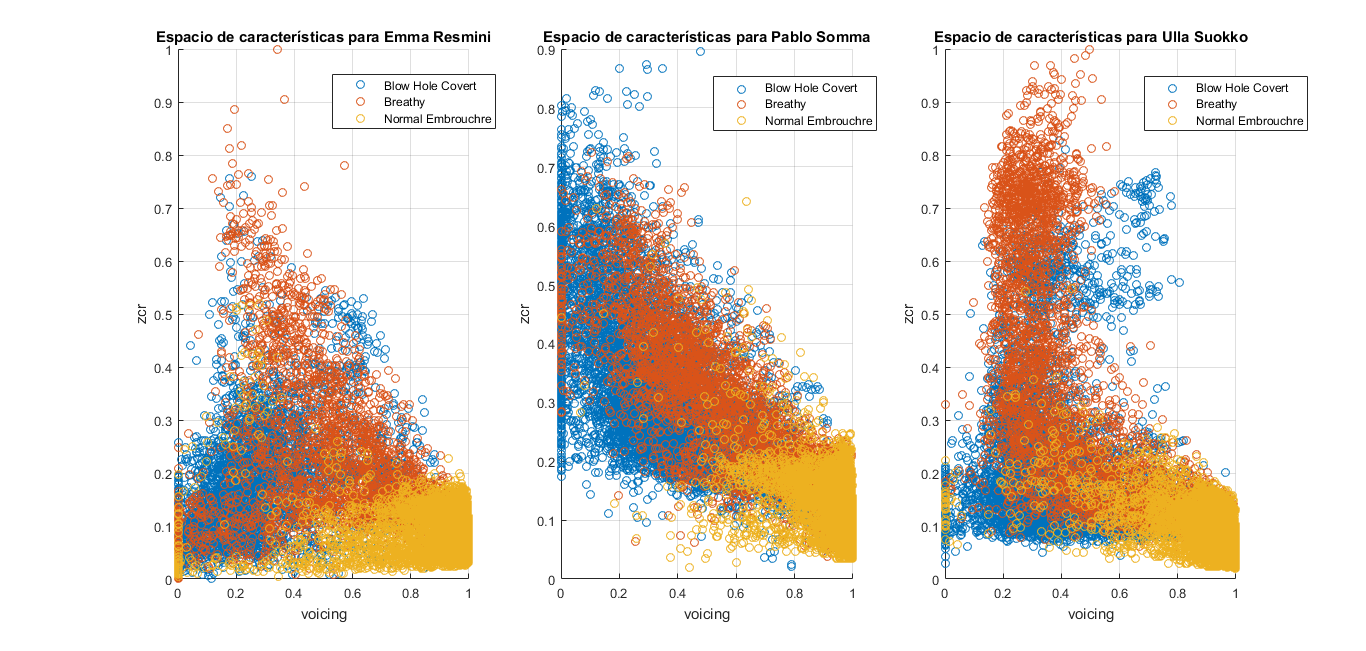
\includegraphics[width=1\textwidth]{histograms_artist} 
%\caption{Espacio de características etiquetado por clases %para cada uno de las interpretaciones.}
%\label{fig:histogramas_artista}
%\end{center}
%\end{figure}

\section*{Conclusiones}

Las caracterísiticas que mejor se comportan en la resolución del problema son las \textit{MFCC's}. Por otro lado \textit{LPC's} de orden $p=26$ y las características de \textit{Voicing} planteadas en la entrega anterior tienen un desempeño similiar.

%----------------------------------------------------------------------------------------
%	BIBLIOGRAPHY
%----------------------------------------------------------------------------------------


\newpage
\bibliographystyle{apalike}
\bibliography{biblio}


%----------------------------------------------------------------------------------------
\end{document}


